\chapter{Background}
\label{chap:back}

In this Chapter, we will review the use of reinforcement learning and Bayesian optimization in robotics, using simulation information to learn faster on hardware and learning the mismatch between the dynamics in simulation and hardware. We also give a short introduction of other policy search methods in literature, which might benefit from simulation information.


\section{Reinforcement Learning}
\label{sec:dp}

Let us consider a controller (agent) that interacts with a process (environment) through a action, which changes the state of the process and generates a reward (feedback from the environment) (Figure \ref{fig:rl}). The controller observes the new state and the reward, and the whole process repeats. The behaviour of the controller is determined by a policy that maps the process state to an action. The process follows a stochastic or deterministic dynamics model which determines how the state changes as a result of actions. 

\begin{figure}[t]
    \centering
    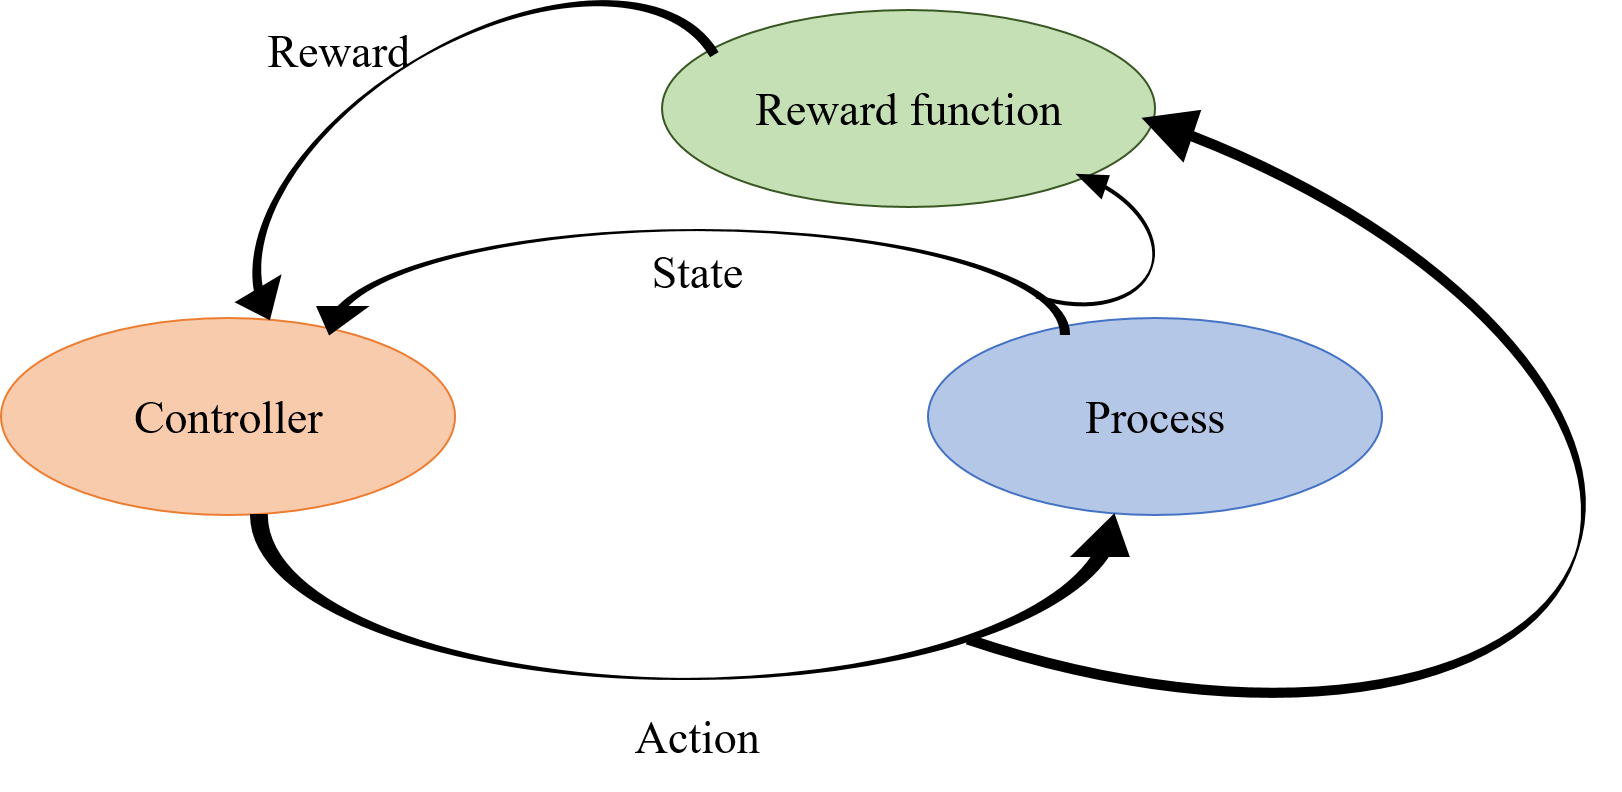
\includegraphics[width=0.7\textwidth]{img/reinforcementLearning.png}
    \caption{The interaction between the controller, process and reward function in dynamic programming and reinforcement learning.}
    \label{fig:rl}
\end{figure}

The goal of reinforcement learning is to find an optimal policy that maximizes the (expected) return, consisting of the (expected) cumulative reward over the course of this interaction, called the value function. This framework can be used to address problems from a variety of fields, e.g., automatic control, artificial intelligence, operations research, and economics.

%\AR{Add RL/DP equations from a standard reference to get notations right}
We assume a discrete-time process and denote the
current time step by $k$. The transition model $p$ is given by a probability distribution conditioned on the current state and current action. We assume a Markov decision process, where the distribution over the next state only depends on the previous state and actions.
\begin{equation}
    s_{k+1} \sim p(s_{k+1}|s_k,u_k)
\end{equation}
where $u_k \in \R^M$ denotes the current action, and $s_k, s_{k+1} \in \R^N$
denote the current and the next state respectively. We furthermore
assume that actions are generated by a policy
\begin{equation}
    u_k \sim \pi_{\theta}(u_k|s_k)
\end{equation}
which is modeled as a probability distribution conditioned on the current state. This lets us naturally include exploratory actions in the policy. The policy is parameterized by some policy parameters $\theta \in \R^M$. Over one episode, the sequence of states and actions forms a trajectory, denoted by $\xi = [s_{0:H}, u_{0:H}]$ where H
denotes the length of the episode. At each instant of time,
the learning system receives a reward (or cost for minimization) denoted by $r(s_k, u_k) \in \R$.

The objective of policy search algorithms is to maximize the expected return of a trajectory, as a function of the policy parameters $\theta$. We assume no-discounting in all our formulations, but discounting factors that weigh future costs lower than the current cost could be added.

\begin{equation}
    J(\theta) = \mathds{E}[\sum_{k=0}^H r_k]
\end{equation}

In general, for each considered policy $\pi_{\theta}$ , a
state-value function $V_\pi(s)$, and a state-action value function (Q-function) $Q_\pi(s,u)$ can be defined as
\begin{align}
    V_\pi(s) = \mathds{E}[\sum_{i=k}^H r_i | s_k = s] \\
    Q_\pi(s, u) = \mathds{E}[\sum_{i=k}^H r_i | s_k = s, u_k = u]
\end{align}
Note, that we can define the expected return in terms of the state-value
function by
\begin{equation}
    J(\theta) = \int_s p(s_0)V_\pi(s_0) ds_0
\end{equation}
where $p(s_0)$ is the probability of $s_0$ being the initial state of an episode.

In the presence of a model, one of the widely used optimal control methods in robotics are dynamic programming algorithms, which can be considered a part of reinforcement learning. Popular dynamic programming methods include value iteration or policy iteration, which are iterative methods that are guaranteed to converge to the global optimum \citep{bertsekas1995neuro}. However, dynamic programming methods do not scale to higher dimensional problems, leading to a ``curse of dimensionality". For example, value iteration converges to the true value function in polynomial time in the number of states and actions \citep{sutton1998reinforcement}. This raises concerns about generalizing to higher dimensions, and especially for continuous action and states. To deal with this, approximate dynamic programming approaches have been suggested, for example, \cite{atkeson2007randomly} randomly sample over actions in a continuous space to avoid discretizing actions. \cite{whitman2009control} break down the problem of controlling a 5-link biped into  4 simpler, lower-dimensional problems and solve each separately. 

Alternatively, in the absence of a model, function approximators can be used to learn the value function and Q-function, resulting in feasible methods even for higher dimensions and continuous action states, example SARSA and Q-learning  \citep{busoniu2010reinforcement}. However, this can result in biases in the estimate of the value function, especially with limited data. Unfortunately, in the general case, since these methods depend on their previous estimate of the target to generate the next solutions, they have an inherent bias based on their initial estimate. Coming up with an appropriate function approximator is a non-trivial problem and can involve using prior knowledge that might not be available, especially for model-free RL. Despite its short-comings, function approximators like deep neural networks have been shown to produce very impressive results in high dimensional control problems. We will talk more about these in Section \ref{sec:deepRL}

Policy search methods avoid the problem of approximating the value function or the Q-function by directly searching for an optimal control policy that maximizes the expected return. For a general problem, the optimization criterion may be a non-differentiable function, with multiple local optima. This means that global, gradient-free optimization techniques are more appropriate than local, gradient-based techniques. Some successful techniques include covariance-matrix adaptation \citep{hansen2006cma}, Bayesian optimization \citep{BOtutorial2016} and cross-entropy optimization \citep{rubinstein1999cross}. We primarily use Bayesian optimization in this work, and we describe that next.
%\AR{Mention a few more policy search works like PILCO, reinforce, etc.}

\section{Bayesian Optimization for Robotics}

In this section, we will provide a basic introduction of Bayesian optimization (BO) and Gaussian processes. This will be followed by a survey of BO for policy search in robotics and in particular, using BO with trajectory information.

\subsection{Bayesian Optimization and Gaussian Processes}
Bayesian optimization (BO) is a framework for sample-efficient black-box and gradient free global search. It was introduced by \cite{jones1998} and originally was referred to as Efficient Global Optimization. 
Recent tutorials like  ~\cite{BOtutorial2016} and ~\cite{BOtutorial2010} provide a  comprehensive overview. Here, we will summarize the basic background for Bayesian optimization to establish notation that will be used in the following sections.

The goal of BO is to find $\pmb{x}^*$ that optimizes an objective function $f(\pmb{x})$, while executing as few evaluations of $f$ as possible. 
The class of functions is not restricted to continuous or smooth functions and hence BO can optimize non-differentiable functions. Little or no a-priori knowledge about $f$ is necessary, but if available, prior knowledge can be incorporated (as we will discuss shortly).

The optimization starts with a prior roughly capturing the prior uncertainty over the value of $f(\pmb{x})$ for each $\pmb{x}$ in the domain. If no prior knowledge is available, this prior can be uninformed and updated with data. As points are sampled, these are included into the estimate of $f(\pmb{x})$, giving an approximate model based on data seen so far. An auxiliary optimization function, called the \textit{acquisition function}, is used to sequentially select points  $\pmb{x}_n$ to sample next, based on the current model of $f(\pmb{x})$. $f(\pmb{x}_n)$ is then evaluated and added to the sampled points. The aim of the acquisition function is to automatically balance exploration and exploitation: select points for which the posterior estimate of the objective $f$ is promising, while also decreasing the uncertainty about $f$. An example of BO is shown in Figure \ref{fig_bo_illustration}. 

\begin{figure}[t]
\centering
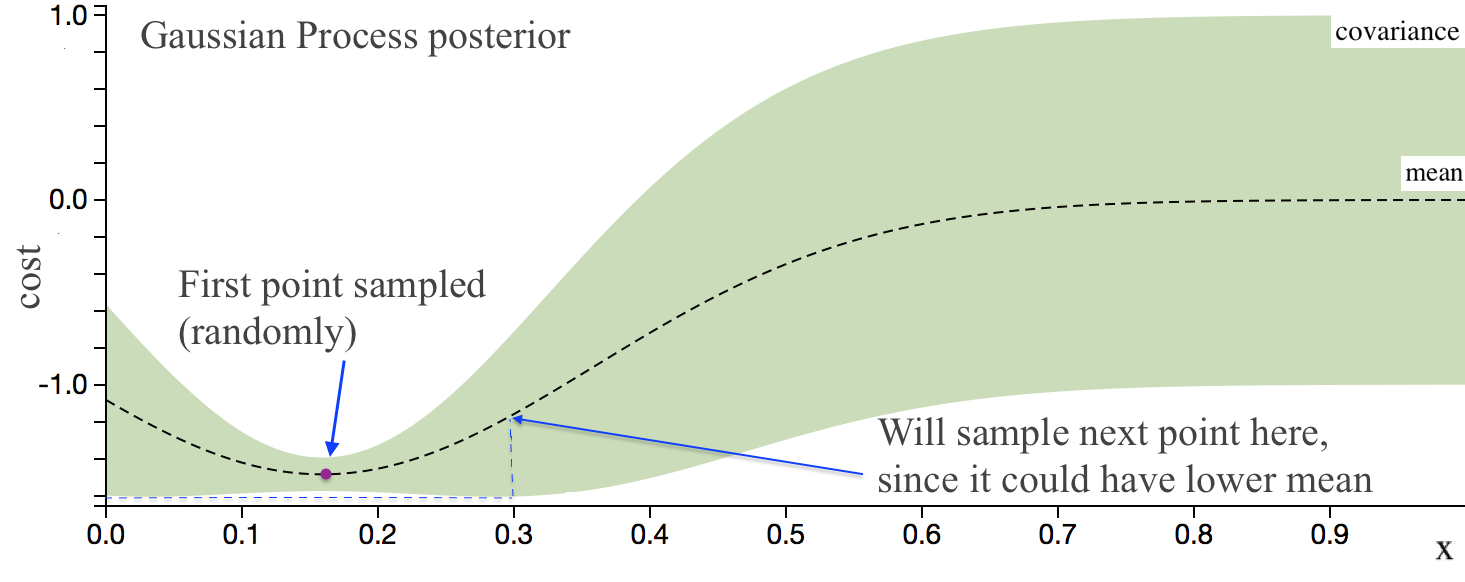
\includegraphics[width=0.75\textwidth]{img/bo_first_point.png}
\vspace{4px}
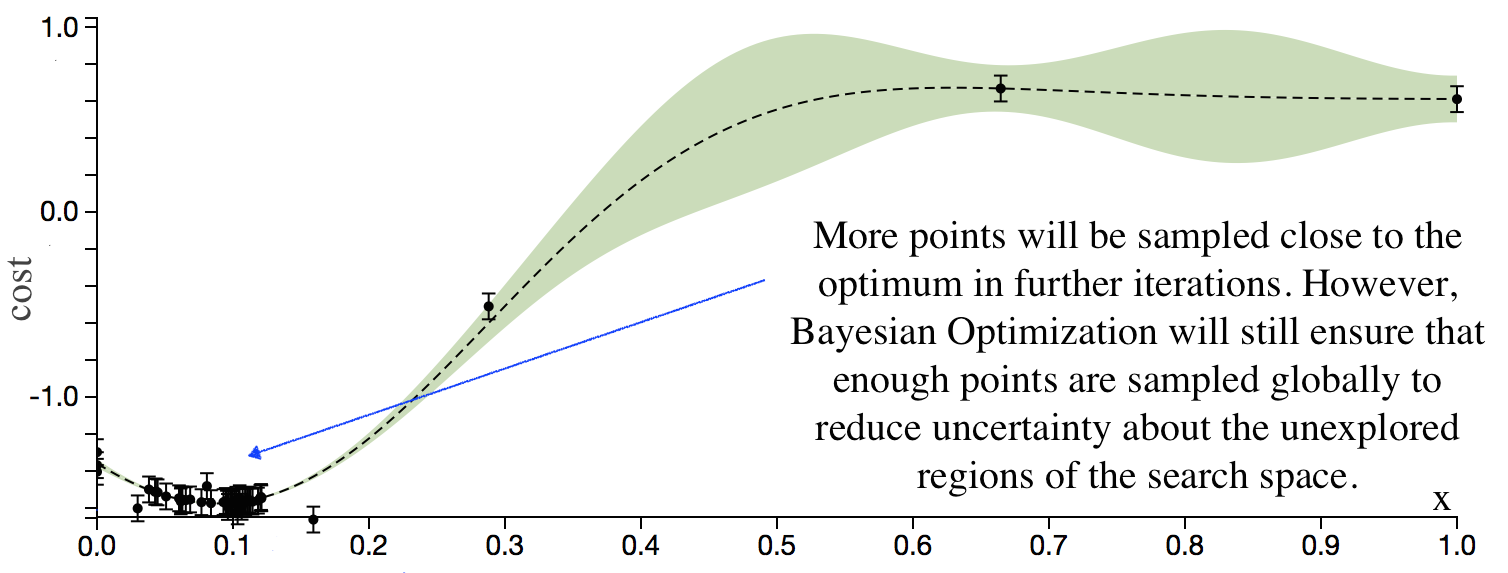
\includegraphics[width=0.75\textwidth]{img/bo_later_points.png}
\caption{\small{Bayesian Optimization posterior for a 1D function. Acquisition function computes the location of points to sample, taking into account both estimated mean and variance (uncertainty).}}
\label{fig_bo_illustration}
\end{figure}

Expected Improvement (EI) function is commonly used as an acquisition function. EI selects $\pmb{x}$ to maximize expected improvement over the value of the best result obtained so far ~\citep{mockus1978ei}. For maximization problems:
\begin{align}
&EI(\pmb{x}) =
\begin{cases}
\big[f(\pmb{x}^+) \!-\! \mu(\pmb{x})\big] \Phi(Z) + \sigma(\pmb{x}) \phi(Z) & \text{if } \sigma(\pmb{x})\!>\!0 \\
0 & \text{ otherwise}
\end{cases} 
\end{align}
where $ \pmb{x}^+ = \argmax_{x_i \in x_{1:t}} f(\pmb{x}_i) $, $\quad Z = (f(\pmb{x}^+) \!-\! \mu(\pmb{x})) / \sigma(\pmb{x})$. 

$\pmb{x}_i$ are points for which objective $f$ has been evaluated so far, $\mu,\sigma$ are posterior mean, variance; $\phi, \Phi$ are PDF and CDF of standard normal distribution. In all our experiments, we use EI as the acquisition function, as it doesn't have any hyperparameters to tune.

Another frequently used acquisition function is Upper Confidence Bound (UCB) or, for minimization problems, Lower Confidence Bound (LCB)~\citep{srinivas2009gpucb}. LCB balances the mean $\mu$ and variance $\sigma$ of the posterior by selecting points which minimize 
\begin{equation}
\label{eq:lcb}
    LCB(\pmb{x}) = \mu(\pmb{x}) - \alpha \sigma(\pmb{x})
\end{equation}

While there can be many ways of modelling $f(\pmb{x})$, we describe a specific non-parametric way of describing $f(\pmb{x})$ using a Gaussian Process (GP). A Gaussian Process is defined by a set of random variables that are jointly Gaussian. It can be completely specified by its mean function and covariance function. 
\begin{align}
f(\pmb{x}) \sim \mathcal{GP}(\mu(\pmb{x}), k(\pmb{x}_i, \pmb{x}_j)),
\end{align}
with mean function $\mu(\pmb{x})$ and kernel $k(\pmb{x}_i, \pmb{x}_j))$. 
\begin{align}
   \mu(\pmb{x}) = \mathds{E}[\pmb{x}] \\
   k(\pmb{x}_i, \pmb{x}_j)) = \mathds{E}[(f(\pmb{x}_i)-\mu(\pmb{x}_i))(f(\pmb{x}_j)-\mu(\pmb{x}_j))]
\end{align}
 %This means that $(f(\pmb{x_1}), f(\pmb{x_2})) \sim \mathcal{N}(\pmb{\mu}, \Sigma)$. To maintain consistency, the marginal distributions are also required to be Gaussian, ie, $f(\pmb{x_1}) \sim \mathcal{N}(\mu_1, \Sigma_{11})$.  Notice that the consistency requirement is automatically fulfilled if the covariance function specifies entries of the covariance matrix.

Assuming Gaussian noise with variance $\sigma^2_{noise}$ on our measurements $y_i$, 
\begin{equation}
    \pmb{y}_i = f(\pmb{x}_i) + \epsilon_{\mathcal{N}(0, \sigma^2_{noise})}
\end{equation}
Gaussian Process conditioned on sampled points represents a posterior distribution for $f$. After evaluating $f$ at points $x_1,...,x_t$ the predictive posterior $P(f_{t+1} | \pmb{x}_{1:t}, \pmb{y}, \pmb{x}_{t+1}) \sim \mathcal{N}\big(\mu_t(\pmb{x}_{t+1}), cov_t(\pmb{x}_{t+1})\big)$ can be computed in closed form with mean and covariance:
\begin{align}
\mu_t(\pmb{x}_{t+1}) = \pmb{k}^T [\pmb{K} + \sigma^2_{noise} \pmb{I}]^{-1} \pmb{y} \quad \quad \quad \\
cov_t(\pmb{x}_{t+1}) = k(\pmb{x}_{t+1}, \pmb{x}_{t+1}) - \pmb{k}^T [\pmb{K} + \sigma^2_{noise} \pmb{I}]^{-1} \pmb{k},
\end{align}
where $\pmb{k} \in \R^t$, with $\pmb{k}_i=k(\pmb{x}_{t+1}, \pmb{x}_i)$; $\pmb{K} \in \R^{t \times t}$ with $\pmb{K}_{ij} = k(\pmb{x}_i, \pmb{x}_j)$; $\pmb{I}$ is an identity $\in \R^{t \times t}$, and $\pmb{y}$ is a vector of values obtained after evaluating $f(\pmb{x}_1), ..., f(\pmb{x}_t)$. More details can be found in~\cite{GPsMLBook}.

The prior mean function $\mu(\pmb{x})$ can be set to $0$ if no relevant domain-specific information is available. The kernel $k(\pmb{x}_i, \pmb{x}_j)$ encodes how similar $f$ is expected to be for two inputs $\pmb{x}_i, \pmb{x}_j$. 
The value of $f(\pmb{x}_i$) has a significant influence on the posterior value of $f(\pmb{x}_j)$, if $k(\pmb{x}_i, \pmb{x}_j)$ is large. The Squared Exponential (SE) kernel is a commonly used similarity metric:
\begin{equation}
k_{SE}(\pmb{x}_i, \pmb{x}_j) = \sigma_k^2 \exp\Big(- \frac{1}{2 \pmb{l}^2} \|\pmb{x}_i - \pmb{x}_j\|^2 \Big),
\end{equation}
where $\sigma_k^2, \ \pmb{l}^2$ denote signal variance and a vector of length scales respectively; $\sigma_k^2, \ \pmb{l}^2$ are called `hyperparameters' in BO literature. It is possible to adjust these automatically during optimization to learn the overall signal variance and how quickly $f$ varies in each input dimension. %Squared Exponential kernel is a special case of a more general class of Mat\'ern kernels~\citep{stein1999interpolation}.


\subsection{Bayesian optimization for policy search}
 As described in Section \ref{sec:dp} policy search circumvents the need to approximate value functions by directly searching for policies that maximize the expected return $J(\theta)$.
 \begin{equation}
    J(\theta) = \mathds{E}[\sum_{k=0}^H r_k]
\end{equation}
The optimal policy parameters $\theta^*$ are defined as
\begin{equation}
    \theta^* = \argmax J(\theta)
\end{equation}

This optimization can be solved sample-efficiently using Bayesian optimization. In this setting, the parameters $\mathbf{x} = \theta$ and the reward/cost function $f = J$. BO samples different policy parameters, executes the policy, and obtains the reward of the episode. This is then used to update the model of $f$ and used to choose the next policy to sample using the acquisition function. It is worth noting that while usually function approximators in reinforcement learning are over states, BO is building an approximation over policies. This way, it is directly searching for the optimal policy that leads to the maximum reward with a fixed initial state distribution. This circumvents building a model over the whole state space, but depends on a specific initial condition distribution. %However, as explained before, such assumptions are common in policy search literature.


\subsection{Bayesian optimization for legged robots}

Bayesian optimization has been used in robotics, usually to tune parameters of controllers, cost functions or planners. The advantage of using a global search framework like BO is that globally optimal policies can be discovered. These may perform better than human hand-designed policies as well as locally optimal solutions. As shown in~\cite{englert2016combined}, the alternative of using Reinforcement Learning (RL) algorithms for policy search might not discover global optima reliably. \cite{frean2008using} use BO to optimize parameters of a neural network controller for a two-link pendulum on a cart. \cite{marco2017virtual} solve the problem of balancing a pole on a real inverted pendulum, by optimizing the cost function for a LQR controller. Authors also propose a way of trading-off simulation and hardware experiments to optimally switch between hardware and simulation for experiments. \cite{martinez2007active} learn the policy for planning the path of a simulated robot that minimizes the uncertainty in its environment.

The most prominent works using Bayesian Optimization for locomotion controllers include \cite{lizotte2007automatic}, \cite{tesch}, \cite{cully2015robots} and \cite{calandra17thesis}. These works typically involve simpler to control robots or smaller bipeds than ATRIAS. \cite{lizotte2007automatic} use AIBO quadrupeds, \cite{tesch} use snake robots, \cite{cully2015robots} use hexapods and \cite{calandra2016bayesian} use a small biped.  \cite{tesch} optimize 3 parameters for a open-loop parametric controller that generates trajectories for a 16 degree of freedom snake robot. The generated solutions find fast moving gaits of about $0.13m/s$ in about 10-40 trials, depending on the difficulty of the task. Such performance was hard to achieve with hand-tuned parameters. \cite{lizotte2007automatic} use BO to optimize open-loop gait parameters for a AIBO robot to maximize velocity and smoothness of movement. They find that the Bayesian optimization
approach not only outperformed previous techniques, but used drastically
fewer evaluations.

%While quadrupeds, hexapods and snake robots can do dynamic gaits, the percentage of time spent dynamically is small as compared to the time spent statically stable. On the other hand, ATRIAS is a highly dynamic robot due to its point feet, and it cannot be statically stable, except in double-stance on a boom. This makes the optimization harder, as the system is unstable leading to discontinuities in cost functions.

\cite{calandra2016bayesian} use BO for optimizing gaits of a 4 dimensional controller on a small biped on a boom. They report needing 30-40 samples for finding walking gaits for a finite-state-machine based controller. This controller consists of 4 threshold parameters that switch the states of a finite-state-machine cycling between stance and swing for each leg. Optimizing a higher-dimensional controller, which is needed for more complex robots and tasks, might prove to be even more challenging. The learning could be especially difficult if a significant number of the points/parameters sampled would lead to unstable gaits and falls. Such samples might result in eventual wear and breakage of the robot hardware (even if care is taken to prevent actual falls). Hence, there is a need to either limit search spaces to ``safe" points, or bias the search towards such points. 

\cite{cully2015robots} tabulate best performing points in simulation versus their average score on a behavioural metric for a hexapod robot. This metric then guides BO to quickly find behaviours that can compensate for damage of the robot. The search on hardware is conducted in behaviour space, and limited to pre-selected ``successful" points from simulation.  This helps make their search faster and safer on hardware.   However, if an optimal point was not pre-selected,  BO cannot sample it during optimization, losing global optimality guarantees.  ``Best points" are cost-specific, so the map needs to be re-generated for new cost functions.

Our proposed method generalizes to highly dynamic behaviours and discontinuous cost functions, while maintaining the global guarantees of BO. We also bias our search towards sampling points successful in simulation (but not exclusively), leading to a sample-efficient and safer search.

\subsection{Incorporating behavior information in Bayesian Optimization}

Adding prior knowledge based on behavior of controllers is a promising avenue to speed up optimization. In higher dimensions, the performance of BO typically degrades, as discussed in \cite{localBO17}. Incorporating domain knowledge, in the form of behavior might speed up optimization in such cases.

Domain knowledge can be incorporated in the form of trajectory information. If we could query the resultant trajectory of each controller, the problem of optimizing the cost would be trivial, as can be expected. To elaborate, consider a Markov Decision Process starting from a state $s_0$, consisting of states $s$ and actions $u$, that follow a transition function $p(s_{k+1}|s,u)$ at time step $k$. Here $p$ defines the probability of transitioning to state $s_{k+1}$ given current state $s$ and taking action $u$. %A typical reinforcement learning problem is characterized reward function $R(x,u,x')$ and a policy $P_\pi(u|x,\theta)$ that maps states to actions,  given some parameters $\theta$. 
Bayesian Optimization, in the classic setting, studies episodic RL which looks at rewards at the end of the execution, or the value of a trajectory. Consider a trajectory $\xi = (s_0, u_0, \cdots , s_H, u_H)$. The probability of sampling this trajectory is
\begin{equation}
    P(\xi|\theta) = P(s_0) \prod_{k=0}^H P(s_{k+1}|s_k,u_k)P(u_k|x_k,\theta)
\end{equation}
The cumulative reward of a trajectory is given as
\begin{equation}
    R(\xi) = \sum_{k=0}^{H-1} R(s_{k+1}, u_{k}, x_{k})
\end{equation}
The expected return of a parameter set $\theta$ then becomes 
\begin{equation}
    J(\theta) = \int R(\xi) P(\xi|\theta) d\xi
\end{equation}

If we can query each trajectory $\xi$ for every controller $\theta$, the cost $J(\theta)$ is perfectly known and the uncertainty $\sigma$ is 0.

%The expected return could itself be a vector consisting of different aspects of a trajectory, for example, distance walked, average speed, cost of transport, etc. The overall cost is a combination of these:
\begin{equation}
    f(\theta) = J(\theta)^Tw
\end{equation}
where $w \sim \mathcal{N}(0, \Sigma_p)$.

%If we fit a GP to this linear setting, the mean and covariance functions become
\begin{align}
    E[f(\theta)] = J(\theta)\\
    E[f(\theta),f(\theta')] = J(\theta)^T \Sigma_p J(\theta)
\end{align}
%If $J(\theta)$ is a scalar, we can determine the the fitness or cost of each controller parameter uniquely in the second trial. 
The UCB acquisition for the posterior (similar to Equation \ref{eq:lcb}) is
\begin{align*}
    \mu(\theta) = J(\theta)\\
    \sigma(\theta) = k(x_2,x_2)-k(x_2,x_1)k(x_1,x_1)^{-1} k(x_1,x_2) = 0 \\
    UCB(\theta) = \mu(\theta) + \alpha \sigma(\theta) = J(\theta)^Tw \\
    \theta_{next} = \argmax_{\theta} UCB(\theta) = \argmax_{\theta} J(\theta)
\end{align*}
$\sigma(\theta) = 0$ is an intuitive result, as for a deterministic setting, there is no uncertainty about the posterior mean of any policy $\theta$. It is exactly equal to $J(\theta)$. Optimizing the acquisition function is equivalent to optimizing the cost. Although it can be difficult to optimize such a function globally, there is no real advantage to using Bayesian optimization anymore. Optimizing the acquisition function can typically need a very large number of samples, which are assumed to be much cheaper than evaluating a policy in BO. However, in the current case, sampling policies for optimizing the acquisition function is just as costly as sampling the actual cost. 
However, this is impossible for a system without unrolling every possible $\theta$ for a controller, which can be prohibitively large number of points. To overcome this, several alternative solutions to evaluating $J(\theta)$ for each point exist in literature.

\cite{wilson2014using} prove an upper bound on the expected improvement of polices as a function of trajectories induced by these policies. 
\begin{align}
%    |J(\theta_i) - J(\theta_j)| = |\int R(\xi)P(\xi | \theta_i) d\xi - \int R(\xi)P(\xi | \theta_j)| d\xi \\
%     = |\int R(\xi) (P(\xi | \theta_i) - P(\xi | \theta_j))| d\xi \\
%     \leq  \int | R(\xi) (P(\xi | \theta_i) - P(\xi | \theta_j))| d\xi \\
   |J(\theta_i) - J(\theta_j)|  \leq  Rmax \int | P(\xi | \theta_i) - P(\xi | \theta_j)| d\xi
\end{align}
The difference between expected returns is upper bunded by the maximum reward per trajectory $Rmax$, and the variational difference in trajectories induced by each policy. Using Pinsker's inequality, and using the fact that $|J(\theta_i) - J(\theta_j)| = |J(\theta_j) - J(\theta_i)|$  this can be written as
\begin{align}
    |J(\theta_i) - J(\theta_j)| = Rmax \sqrt{2} (\sqrt{KL(P(\xi|\theta_i)||P(\xi || \theta_j))} + \sqrt{KL(P(\xi|\theta_j)||P(\xi || \theta_i))} )
\end{align}

The authors use this symmetric positive definite result to construct a kernel defined as:
\begin{align}
D_{ij} = \sqrt{KL(P(\xi|\theta_i)||P(\xi || \theta_j))} + \sqrt{ KL(P(\xi|\theta_j)||P(\xi || \theta_i))} \\
K(\theta_i, \theta_j) = \exp(-\alpha * D_{ij})
\end{align}

This new Behavior Based Kernel (BBK) uses the KL distance of trajectories induced by the evaluated policies to calculate kernel distances. A kernel constructed to use behavior-based similarity offered an improvement over a standard SE kernel. However, BBK required obtaining trajectory data every time kernel values $k(\pmb{x}_i, \pmb{x}_j)$ were evaluated. This would not be tractable when optimizing locomotion controllers, as it would need a full evaluation to determine the kernel distance (similar to the problem we described above). The authors suggest combining BBK with a model-based approach to overcome this difficulty by learning a transition model for the problem. But building a reliable model might need several data points, and building good models with few data points is an interesting research question in itself.

\cite{cully2015robots} build a behavior map based on the simulation of controllers. They overcome the problem of building models of the robot from hardware data, but rely on behavior transfer between simulation and hardware. However, rather than using behavior as part of the kernel, as in \cite{wilson2014using}, they build a look-up map between behavior and ``successful" controllers. They then search in the low-dimensional behavior space, among the pre-selected controllers from simulation. Though this leads to a highly sample-efficient search and potentially safe samples, this method cannot search beyond the pre-selected points, and hence loses the global guarantees of BO.

\cite{marco2017design} design a kernel for LQR control assuming a quadratic cost and a one-dimensional linear system model. For such a problem, they show improvements in cost within 3 trials. It is unclear how this approach would scale to higher dimensional problems and other controllers.

Our approach constructs an informed kernel that incorporates behavior-based similarity, in a manner that ensures $k(\pmb{x}_i, \pmb{x}_j)$ can be obtained efficiently when running BO. We pre-calculate locomotion-specific features on a high-fidelity simulator by running short simulations, enabling us to efficiently calculate the kernel distances during optimization. Our feature transform also biases the search towards high performing points in simulation, which have a higher chance of being stable on hardware than randomly selected points. In this manner, we try to incorporate behavior information from simulation, as also was proposed in \cite{cully2015robots}, but maintain global guarantees of BO.



\section{Reinforcement learning for bipedal robots}
Reinforcement learning (RL) has been widely applied to robotics problems, including simulations and hardware of manipulation, locomotion, perception problems. The widespread use of RL makes it hard to review all works in robotics, hence we will focus largely on RL for bipedal locomotion. 

Some of the applications of RL on bipedal robots include, \cite{tedrake2004stochastic}, \cite{morimoto2005poincare}, \cite{benbrahim1997biped} and \cite{nakanishi2004learning}.
\cite{tedrake2004stochastic} started with a passively stable 3d biped and added ankle actuation. With simplifications, like decoupling the roll and sagittal degrees of freedom, they approximate a value function and the control policy using linear function approximators. This system was shown to learn to walk in a very short time. \cite{morimoto2005poincare} modulate the via-points of reference trajectories of hip and knee joints of a 5-link biped, by learning a value function, control policy and a Poincar\'e section of the robot. The policy-gradient method, aided by the Poincar\'e model, found robust walking solutions in 100 trials on a complex robot hardware. \cite{benbrahim1997biped} use a central-pattern generator (CPG) based controller, whose parameters are tuned online using an actor critic method. However, the robot had to be externally supported with a ``walker" to aid stability. \cite{nakanishi2004learning} use a rhythmic dynamic movement primitive to learn an initial gait from locomotion and adapt the frequency of oscillation using RL on a 5-link biped.

Another popular approach employing RL or DP in robotics is using it to learn the Center of Mass (CoM) trajectory, and follow it using optimization based Inverse Dynamics. \cite{kormushev2011bipedal} use RL to reduce the energy consumption by learning a variable-height CoM trajectory, with a evolving policy parametrization of their policy. The learned CoM trajectory exploits the passive dynamics of the COMAN robot and reduces the overall energy of walking better than the fixed policy parametrizations. \cite{feng2015optimization} use an approximation of dynamic programming, called Differential Dynamic Programming to optimize the CoM trajectory using an inverted pendulum model with ankle torques. Combining this with reactive foot placement in \cite{feng2016robust} results in very a robust walking controller on the ATLAS humanoid robot. An application of approximate dynamic programming for whole-body control of bipedal robots was described in \cite{whitman2009control}. \cite{whitman2009control} break down the problem of controlling a 5-link biped into  4 simpler, lower-dimensional problems - sagittal stance, sagittal swing, coronal stance and yaw control. The coupled dynamics of the simpler models are considered as disturbances. The control policy generated by dynamic programming is robust to perturbations in forward and lateral directions, as well as generalize to different speeds. This was also implemented on the Sarcos humanoid and shown to reject small unknown disturbances while walking.


%\cite{} use differential dynamic programming (DDP) to develop robust controllers applied to a 5-link biped. The differences between hardware and simulation are treated as disturbances that the learned feedback controller is able to reject.
%One of the common control parametrizations used with RL on bipedal robots are central pattern generators (CPGs). 

\subsection{Learning with neural networks in robotics}

Recently, there has been a surge in work using neural networks to control robots, though hardware results on locomotion robots are few. Techniques like deep reinforcement learning however have shown tremendous progress at solving complex manipulation and locomotion tasks in simulation. Recently deep reinforcement learning (DRL) has shown beyond human performance on complex long-horizon games such as Go \cite{silver2016mastering}, even when starting with no human input. Similar progress has been achieved in the domain of continuous control too, dealing with very high dimensional state and action spaces. For example, Deep Deterministic Policy Gradients (DDPG) ~\citep{lillicrap2015continuous} and Trust Region Policy Optimization  (TRPO) ~\citep{schulman2015trust} can solve several control challenges in the Mujoco simulation environment \citep{todorov2012mujoco}. \cite{heess2017emergence} show that a variant of the Proximal Policy Optimization (PPO) \citep{schulman2017proximal} can learn to control a very high degree of freedom humanoid robot in Mujoco, even in very challenging environments. Similarly, \cite{rajeswaran2017towards} use a variant of DDPG to learn to do dexterous manipulation with a high degree of freedom hand in simulation.

While simulation results for deep RL are very impressive, the simulation-hardware gap makes most controllers learned in simulation unsuitable to be implemented on hardware. This is partly because simulations are not perfect representations of real systems, but also because learning approaches often tend to exploit simulation inaccuracies to achieve better performance. High-dimensional neural network policies can approximate arbitrarily complex controllers, but too expensive to optimize directly on hardware. One approach to learn policies in simulation and deploy on hardware is domain randomization \citep{mordatch2015ensemble}. It can be used to learn robust neural network policies in simulation by applying random perturbations to the dynamics and other properties of the simulator. This approach has been applied to manipulation problems \citep{peng2017sim}, as well as quadrupedal locomotion problems \citep{tan2018sim}. However, typical domain randomization can lead to controllers that perform worse than controllers trained without randomization \citep{tan2018sim}, as well as make the learning problem much harder \citep{2018arXiv180800177O} taking over 100 years of simulation time to learn successful policies.   

\subsubsection{Deep Reinforcement Learning for locomotion}
\label{sec:deepRL}

\cite{peng2016terrain} formulate the problem of learning locomotion gaits as a actor-critic Reinforcement Learning with neural networks as function approximators for policy and value functions. The neural network takes as input terrain and robot states, parametrized leaps or steps as output. The input dimensionality is large (83D robot state and a 200D terrain state) and maps to a 29D control space, that operates at a high level, like leaps and steps for the robot, leading to about 570k parameter large network. The outputs from the policy network is fed to a finite state machine which is hand-designed to achieve the goal dictated by the neural network. While highly successful at traversing very uneven terrain, this network needs over 10 million data points to train the network. 
%Such approaches, however, are not data-efficient enough to support learning optimal parameters for locomotion controllers on real hardware. So in our work we are interested in combining sample efficiency of an approach like Bayesian Optimization with the flexibility and scalability of deep neural networks.

\cite{heess2017emergence} use deep reinforcement learning to learn locomotion tasks for a biped, humanoid walker and a quadruped, training the neural network with increasingly difficult terrains. The network takes as input the terrain state and the robot state and directly outputs the torques for each joint. They develop a robust policy gradient method that uses a trust region constraint to restrict the policy update from changing too much, making the policy gradient robust to noise and hyperparameter selection. This results in highly dynamic and robust gaits in simulation, though it is unclear if such policies can be learned on hardware.

To avoid having to learn such policies on hardware directly, \cite{tan2018sim} use domain randomization in simulation to learn robust policies for a quadrupedal robot. They learn two dynamic gaits - trotting and galloping in simulation, and test the trained policies on hardware. The trained policies were able to achieve about the same speed as handcrafted policies, they consumed less mechanical power. While controllers trained with domain randomization had a lower expected return in simulation than those trained without, their performance on hardware was much better. This is expected because robust controllers are typically more conservative, but easily generalizable to different systems.

%\AR{Maybe add a section about other sim to real work in deep rl}

\subsubsection{Guided policy search and related methods}

Guided policy search is a recently popularized method for learning policies for robotic tasks \citep{levine2013guided} using neural networks. It has been applied to learning policies from images for complex manipulation tasks, such as peg-in-hole \cite{levine2016end}, contact-rich tasks like opening doors \cite{levine2015learning}, etc. These networks represent global policies that are initialized by locally optimal policies. On facing new situations, where the local policies fail, a new local policy is initialized and trained to minimize cost and stay close to the global policy. The global policy is now updated to match the local policy. This ensures an increasingly general global policy that stays close to the initial policy, minimizing the ``forgetting" factor for neural networks. 

While there hasn't been work on locomotion on hardware with guided policy search, initializing the network in simulation over perturbed models and implementing on hardware seems straightforward. To enable fast learning on hardware, it might be beneficial to aid the policy gradients from optimal gradient step-size from simulation. This can be done either using natural gradients \cite{peters2006policy} from simulation or a meta-function that predicts gradient step-size \cite{meier2017online}. Aiding gradient descent based on information from simulation can help with sample-efficiency on hardware. This was originally proposed in \cite{abbeel2006using} where exact evaluations were aided with approximate gradients to suggest local improvements. While the exact value of the value function might be different between simulation and hardware, the gradient direction and step-size might have higher probability of transferring. Since learning rates are sensitive to hyper parameters like step-size, learning these in simulation seems straight-forward and beneficial. This can be done in combination with a mismatch-map which predicts the likelihood of transfer between simulation and hardware. If we expect high mismatch, we can use hardware samples to learn the correct learning rate.